% Provenance (never printed): old seconde/premiere S material on the
% atmosphere (water vapour, saturation, cloud formation, the vertical motion
% of air) and enseignement scientifique premiere (water cycle); see
% sources/book2/PROVENANCE.md. Every saturation value, lapse rate,
% condensation level and the lee-wind example are computed in
% figdata/grade-10/clouds.py from the IAPWS saturation curves; the soundings
% are invented examples, said so in the text.
\chapter{Por qué se forman las nubes}\label{ch:g10:why-clouds-form}

En una terraza, un día de verano, hay un vaso de agua con hielo sobre una
mesa. En menos de un minuto, su cara exterior se cubre de gotitas y un cerco
de agua se extiende a su pie. El agua no se ha filtrado a través del vidrio:
ha salido del aire, que se ha enfriado al tocar el vaso frío. Unas horas más
tarde, a kilómetros por encima de la llanura, ocurre lo mismo a gran escala:
burbujas de aire caliente suben, se enfrían y, a cierta altura, el agua que
transportan aparece en forma de esos montones de nube blanca de base plana
llamados cúmulos. Este capítulo explica cuánto vapor de agua puede contener
el aire, por qué se enfría el aire que sube, a qué altura se forman las
nubes, por qué unos días se quedan planas y otros crecen hasta convertirse
en tormentas, y cómo las diminutas gotitas de nube se convierten en lluvia y
en nieve.

\begin{omfigure}
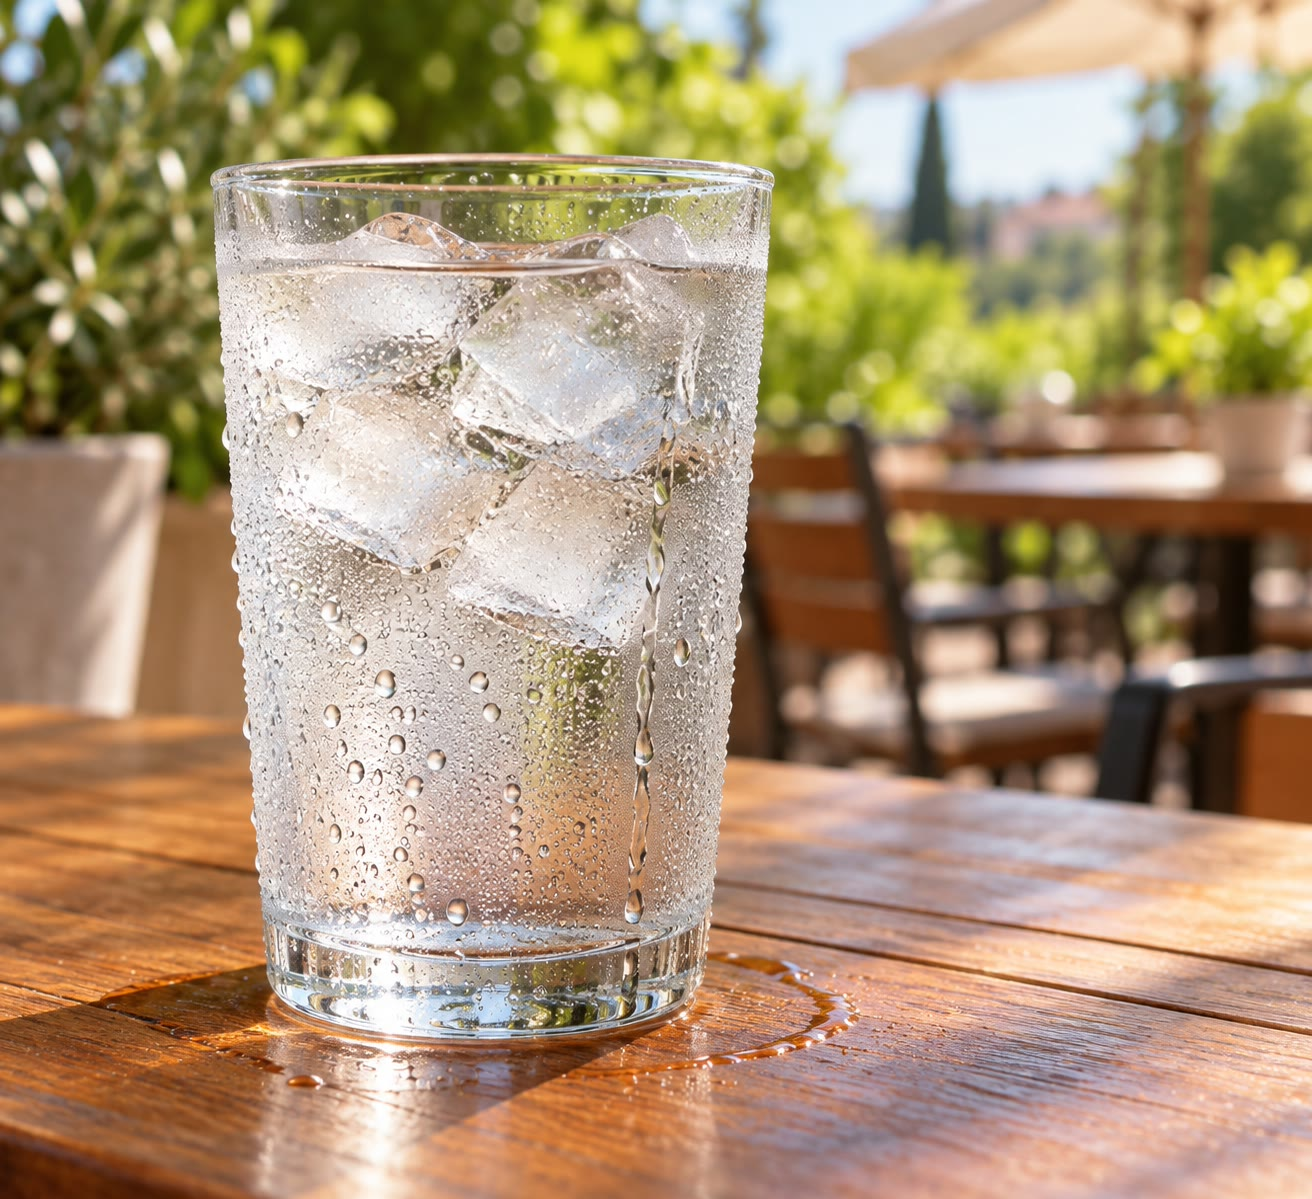
\includegraphics[width=0.5\linewidth]{images/book2/ai/g10-cold-glass.jpg}

{\small Un vaso de agua con hielo en una terraza en verano: en su cara
exterior se forman gotas, allí donde se enfría el aire que toca el vidrio.}
\end{omfigure}

\begin{recall}
Las nubes están formadas por diminutas gotitas de agua o cristales de hielo;
se clasifican en familias según su forma y su altura, y dan lluvia, nieve y
granizo, que se miden con un pluviómetro (Libro 1, año 4). La temperatura
del aire disminuye con la altura en la capa más baja de la atmósfera, por
término medio unos \qty{6.5}{\degreeCelsius} por kilómetro; es el gradiente
térmico vertical, y los frentes separan masas de aire de temperaturas
distintas (Libro 1, año 8). La presión disminuye con la altura (los libros
de física). El agua se evapora y se condensa, y la evaporación absorbe un
\omterm{def:g10:earth-energy-budget:latent-heat}{calor latente} que la condensación devuelve (los libros de física y el
\cref{ch:g10:earth-energy-budget}).
\end{recall}
% ledger: nasa:grc-atmosphere

\section{El vapor de agua y la saturación}

El aire siempre contiene algo de vapor de agua, un gas invisible. Cuánto
puede contener depende sobre todo de su temperatura.

\begin{definition}[Saturación; humedad relativa]\label{def:g10:why-clouds-form:humidity}
El aire está \emph{saturado}\index{saturacion@saturación} cuando contiene la
mayor masa de vapor de agua que puede admitir a su temperatura, su
\emph{contenido de saturación}; todo el vapor de más se condensa en gotitas.
La \emph{humedad relativa}\index{humedad relativa} del aire es su contenido
de vapor de agua dividido entre su contenido de saturación a la misma
temperatura y presión, expresado en porcentaje.
\end{definition}

El contenido de agua del aire se mide aquí en gramos de vapor por kilogramo
de aire seco (\unit{g/kg}): una porción de aire que sube o baja sin ganar ni
perder agua conserva el mismo contenido, aunque se dilate.

\begin{omfigure}
\begin{tikzpicture}
\begin{axis}[omrecord, width=0.88\linewidth, height=6.2cm, xmin=-10, xmax=40,
  ymin=0, ymax=50, xlabel={temperatura (\unit{\degreeCelsius})},
  ylabel={contenido de saturación (\unit{g/kg})}, xtick={-10,0,...,40},
  tick label style={font=\small}, label style={font=\small}]
\addplot[omDef!85!black, thick] table[x=T_C, y=ws_gkg] {figdata/out/grade-10-clouds-sat.dat};
\addplot[only marks, mark=*, mark size=1.8pt, omThm!85!black] coordinates {(28,11.37)};
\addplot[only marks, mark=o, mark size=1.8pt, omThm!85!black] coordinates {(16,11.37)};
\draw[->, omThm!85!black, thick] (axis cs:27.2,11.37) -- (axis cs:16.9,11.37);
\node[anchor=north, font=\footnotesize, omThm!85!black] at (axis cs:28,10.6) {aire a \qty{28}{\degreeCelsius}};
\node[anchor=south east, font=\footnotesize, omThm!85!black] at (axis cs:15.5,12.2) {punto de rocío};
\node[anchor=south east, font=\footnotesize, omDef!85!black, align=right] at (axis cs:31,34) {por encima de la curva:\\el vapor se condensa};
\node[anchor=south west, font=\footnotesize, omDef!85!black] at (axis cs:31,2.5) {no saturado};
\node[anchor=north west, font=\footnotesize, omDef!85!black] at (axis cs:34,31.5) {saturación};
\end{axis}
\end{tikzpicture}

{\small La mayor masa de vapor de agua que puede contener un kilogramo de
aire, en función de la temperatura, a la presión del nivel del mar (sobre
agua líquida; calculada con la norma internacional para el agua). El aire a
\qty{28}{\degreeCelsius} con \qty{11.4}{g/kg} (punto) está lejos de la
\omterm{def:g10:why-clouds-form:humidity}{saturación}; si se enfría sin perder agua, se satura a
\qty{16}{\degreeCelsius} (círculo).}
\end{omfigure}
% ledger: iapws:vapour-pressure, ciaaw:abridged-2024, earth:Mmol, const:R (computed in figdata/grade-10/clouds.py)

La curva sube con fuerza: \qty{3.8}{g/kg} a \qty{0}{\degreeCelsius},
\qty{14.7}{g/kg} a \qty{20}{\degreeCelsius}, \qty{27.2}{g/kg} a
\qty{30}{\degreeCelsius}. Cada \qty{10}{\degreeCelsius} de calentamiento
casi duplican el agua que puede contener el aire. Por eso el aire tropical
puede traer lluvias torrenciales, y por eso el aire de un invierno polar,
incluso \omterm{def:g10:why-clouds-form:humidity}{saturado}, apenas contiene nada.

\begin{definition}[Punto de rocío]\label{def:g10:why-clouds-form:dew-point}
El \emph{punto de rocío}\index{punto de rocio@punto de rocío} del aire es la
temperatura a la que hay que enfriarlo, conservando su contenido de agua y
su presión, para que se sature.
\end{definition}

\begin{method}[Humedad relativa y punto de rocío a partir de una tabla]\label{met:g10:why-clouds-form:table}
\begin{enumerate}
  \item Lee en la tabla el contenido de \omterm{def:g10:why-clouds-form:humidity}{saturación} a la temperatura del aire.
  \item \omterm{def:g10:why-clouds-form:humidity}{Humedad relativa}: divide entre él el contenido de agua del aire.
  \item \omterm{def:g10:why-clouds-form:dew-point}{Punto de rocío}: busca en la tabla la temperatura cuyo contenido de
        \omterm{def:g10:why-clouds-form:humidity}{saturación} es igual al contenido de agua del aire.
\end{enumerate}
\end{method}

\begin{example}[Una mañana de verano]\label{ex:g10:why-clouds-form:morning}
% ledger: iapws:vapour-pressure (values computed in figdata/grade-10/clouds.py)
A \qty{20}{\degreeCelsius}, el aire contiene \qty{11.4}{g/kg}. El
contenido de \omterm{def:g10:why-clouds-form:humidity}{saturación} a \qty{20}{\degreeCelsius} es de \qty{14.7}{g/kg},
así que la \omterm{def:g10:why-clouds-form:humidity}{humedad relativa} es $11.4/14.7 \approx \qty{78}{\percent}$. El
contenido de \omterm{def:g10:why-clouds-form:humidity}{saturación} vale \qty{11.4}{g/kg} a \qty{16}{\degreeCelsius}:
ese es el \omterm{def:g10:why-clouds-form:dew-point}{punto de rocío}. Por la tarde, el mismo aire calentado a
\qty{28}{\degreeCelsius} (contenido de \omterm{def:g10:why-clouds-form:humidity}{saturación} de \qty{24.1}{g/kg}) solo
tiene una \omterm{def:g10:why-clouds-form:humidity}{humedad relativa} del \qty{47}{\percent}, con exactamente la misma
agua.
\end{example}

El vaso del principio está más frío que el \omterm{def:g10:why-clouds-form:dew-point}{punto de rocío} del aire que lo
rodea: el aire que lo toca se enfría por debajo de su \omterm{def:g10:why-clouds-form:dew-point}{punto de rocío} y deja
agua sobre el vidrio. En una noche despejada, la hierba y los techos de los
coches pierden calor radiando infrarrojo hacia el cielo y se enfrían más que
el aire: sobre ellos se forma rocío, o escarcha por debajo de
\qty{0}{\degreeCelsius}. Cuando toda una capa de aire cercana al suelo se
enfría hasta su \omterm{def:g10:why-clouds-form:dew-point}{punto de rocío}, se forman gotitas en el propio aire: es la
niebla.

\begin{omfigure}
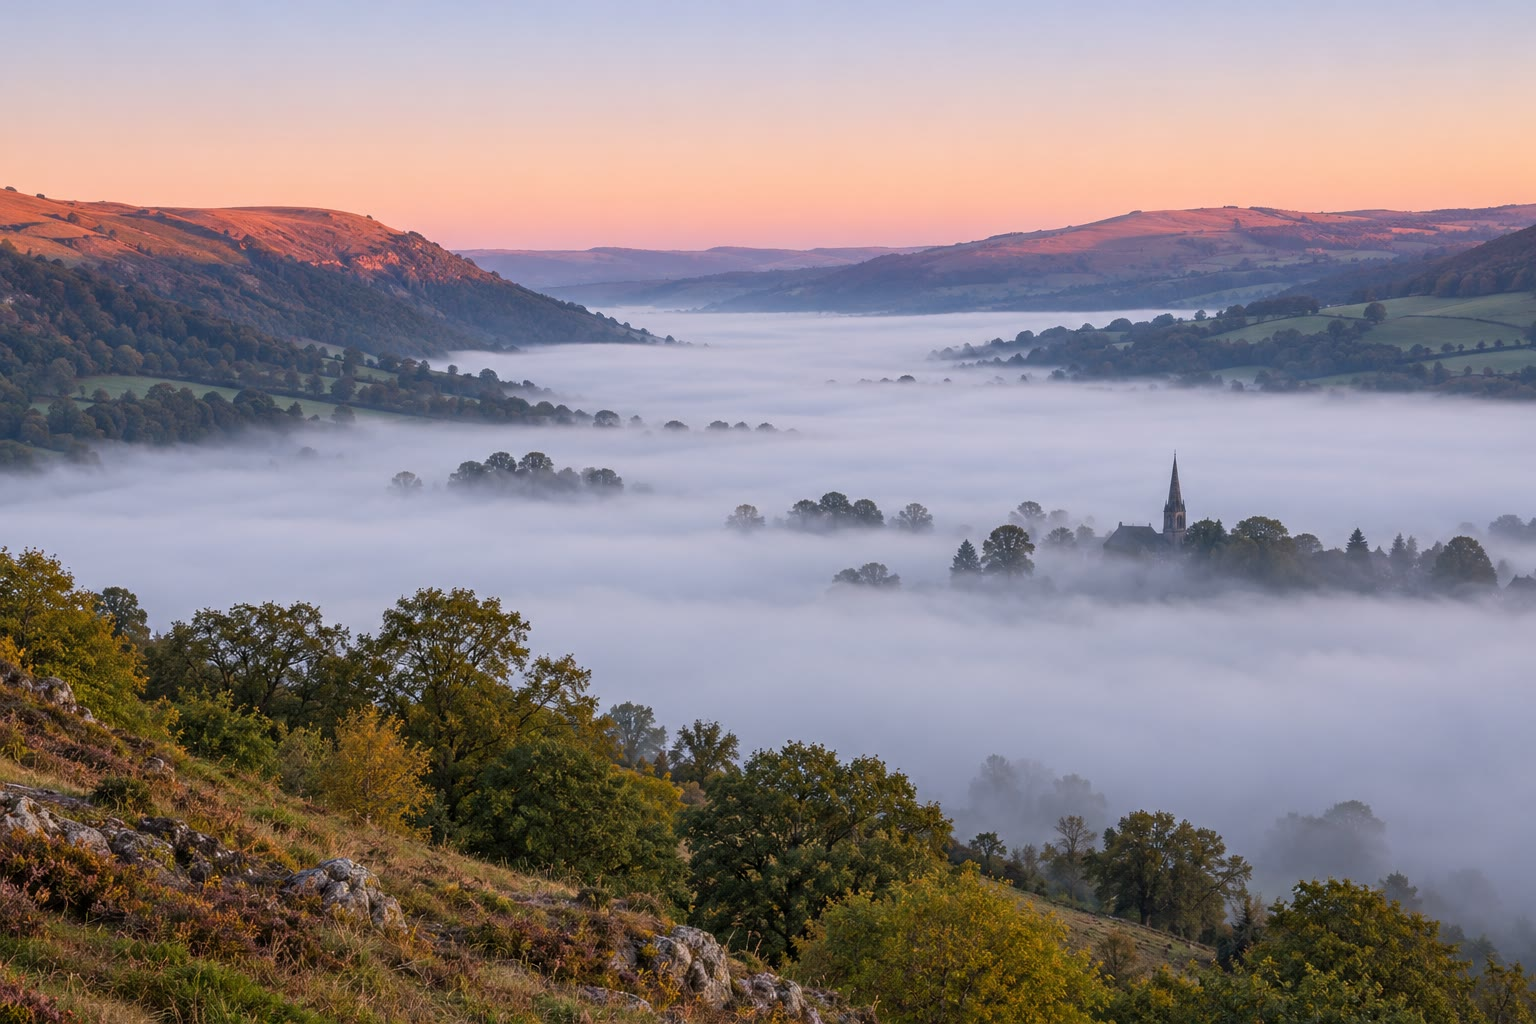
\includegraphics[width=0.75\linewidth]{images/book2/ai/g10-valley-fog.jpg}

{\small Niebla que llena un valle al amanecer. Durante la noche despejada,
el suelo se enfrió, el aire frío descendió hasta el valle y allí se enfrió
por debajo de su \omterm{def:g10:why-clouds-form:dew-point}{punto de rocío}.}
\end{omfigure}

\section{El aire que sube se enfría}

La mayoría de las nubes no se forman porque el aire toque algo frío. Se
forman porque el aire sube. La presión disminuye con la altura; una porción
de aire que sube se dilata, empujando el aire que la rodea, y la energía de
este trabajo la toma de sí misma.

\begin{definition}[Enfriamiento adiabático; gradiente adiabático seco]\label{def:g10:why-clouds-form:adiabatic}
El \emph{enfriamiento adiabático}\index{enfriamiento adiabatico@enfriamiento adiabático}
es el enfriamiento de una porción de aire que se dilata sin intercambiar
calor con su entorno. El ritmo al que se enfría así el aire no \omterm{def:g10:why-clouds-form:humidity}{saturado} que
sube es el \emph{gradiente adiabático seco}\index{gradiente adiabatico seco@gradiente adiabático seco},
cercano a \qty{9.8}{\degreeCelsius} por kilómetro de ascenso; el aire que
baja se calienta al mismo ritmo.
\end{definition}

\begin{proposition}[El gradiente adiabático seco]\label{prop:g10:why-clouds-form:dry-rate}
El \omterm{def:g10:why-clouds-form:adiabatic}{gradiente adiabático seco} es $g/c_p$, donde $g = \qty{9.81}{m/s^2}$ y $c_p
\approx \qty{1005}{J.kg^{-1}.K^{-1}}$ es la energía que calienta un
kilogramo de aire un grado a presión constante: $9.81/1005 \approx
\qty{0.0098}{\degreeCelsius/m}$, es decir, \qty{9.8}{\degreeCelsius/km}.
(Se admite: la demostración corresponde a los libros de física.)
\end{proposition}
% ledger: const:gn, const:R, earth:Mmol (c_p of dry air computed as (7/2)R/M in figdata/grade-10/clouds.py)

El \omterm{def:g10:why-clouds-form:dew-point}{punto de rocío} de la porción también baja a medida que sube, pero
despacio: su contenido de agua no cambia, mientras que la caída de presión
hace que el vapor se sature un poco más fácilmente. El cálculo para el aire
cercano al suelo da unos \qty{1.8}{\degreeCelsius} por kilómetro. Por tanto,
la temperatura de la porción se acerca a su \omterm{def:g10:why-clouds-form:dew-point}{punto de rocío} unos
$9.8 - 1.8 = \qty{8}{\degreeCelsius}$ por cada kilómetro que asciende.
% ledger: iapws:vapour-pressure (dew-point rate computed in figdata/grade-10/clouds.py)

\begin{definition}[Nivel de condensación]\label{def:g10:why-clouds-form:condensation-level}
El \emph{nivel de condensación}\index{nivel de condensacion@nivel de condensación}
de una porción de aire es la altura a la que, al subir, se satura. Por
encima de él, el agua se condensa: el nivel de condensación es la base
plana de las nubes que forma el aire ascendente.
\end{definition}

\begin{proposition}[Altura del nivel de condensación]\label{prop:g10:why-clouds-form:lcl}
El aire que sube desde el suelo con una temperatura $T$ y un \omterm{def:g10:why-clouds-form:dew-point}{punto de rocío}
$T_d$ (en \unit{\degreeCelsius}) se satura aproximadamente a
\[
  z = \frac{T - T_d}{8}\ \text{km} = \qty{125}{m} \times (T - T_d).
\]
\end{proposition}

\begin{proof}
A una altura $z$ (en km), la temperatura de la porción es $T - 9.8\,z$ y su
\omterm{def:g10:why-clouds-form:dew-point}{punto de rocío}, $T_d - 1.8\,z$. Se satura cuando son iguales:
$T - 9.8\,z = T_d - 1.8\,z$, luego $8\,z = T - T_d$ y $z = (T - T_d)/8$ km.
Un octavo de kilómetro son \qty{125}{m}.
\end{proof}

\begin{example}[Un cúmulo de la tarde]\label{ex:g10:why-clouds-form:base}
% ledger: iapws:vapour-pressure (exact ascent computed in figdata/grade-10/clouds.py: 1.51 km)
Por la tarde del día del \cref{ex:g10:why-clouds-form:morning}, el aire
junto al suelo está a \qty{28}{\degreeCelsius} con un \omterm{def:g10:why-clouds-form:dew-point}{punto de rocío} de
\qty{16}{\degreeCelsius}. Las burbujas que suben se saturan a
$125 \times 12 = \qty{1500}{m}$: los cúmulos tienen la base plana a unos
\qty{1.5}{km} de altura. Por la mañana, a \qty{20}{\degreeCelsius}, el mismo
aire se habría condensado a solo $125 \times 4 = \qty{500}{m}$: la base de
las nubes sube a lo largo del día a medida que se calienta el suelo.
\end{example}

\section{Aire estable y aire inestable}

Que una porción que sube siga subiendo depende del aire que la rodea. Una
porción más caliente que su entorno es más ligera que el aire que desplaza y
sube, como un globo aerostático; una porción más fría que su entorno vuelve
a bajar.

\begin{definition}[Aire estable; aire inestable]\label{def:g10:why-clouds-form:stability}
El aire es \emph{estable}\index{aire estable} cuando una porción empujada
hacia arriba se vuelve más fría que el aire que la rodea y, por tanto,
vuelve a bajar hasta donde estaba. Es \emph{inestable}\index{aire inestable}
cuando la porción se vuelve más caliente que el aire que la rodea y sigue
subiendo por sí sola.
\end{definition}

La porción que sube se enfría según el \omterm{def:g10:why-clouds-form:adiabatic}{gradiente adiabático seco},
\qty{9.8}{\degreeCelsius} por kilómetro, mientras no está saturada. Una vez
saturada, se enfría más despacio: la condensación libera \omterm{def:g10:earth-energy-budget:latent-heat}{calor latente} en la
porción. El cálculo da unos \qty{4.7}{\degreeCelsius} por kilómetro en el
aire cálido cercano al suelo, unos \num{5.8} a \qty{0}{\degreeCelsius}, y
más en el aire frío de las capas altas, donde queda poca agua por
condensar; es el gradiente \omterm{def:g10:why-clouds-form:humidity}{saturado}. (Su fórmula se deduce en los volúmenes
universitarios.)
% ledger: nist:water-latent, iapws:vapour-pressure (saturated rates computed in figdata/grade-10/clouds.py)

\begin{method}[¿Es estable este aire?]\label{met:g10:why-clouds-form:stable}
\begin{enumerate}
  \item Averigua a qué ritmo disminuye con la altura la temperatura del aire
        que rodea la porción (el gradiente térmico vertical, obtenido con un
        sondeo en globo).
  \item Compáralo con el ritmo al que se enfría la porción: el gradiente
        seco, unos \qty{9.8}{\degreeCelsius/km}, por debajo de su \omterm{def:g10:why-clouds-form:condensation-level}{nivel de
        condensación}; el gradiente \omterm{def:g10:why-clouds-form:humidity}{saturado}, unos
        \qty{5}{\degreeCelsius/km}, por encima.
  \item Si el entorno se enfría más despacio que la porción, la porción
        acaba más fría: \omterm{def:g10:why-clouds-form:stability}{estable}. Si se enfría más deprisa, la porción acaba
        más caliente: \omterm{def:g10:why-clouds-form:stability}{inestable}. Una capa en la que la temperatura
        \emph{aumenta} con la altura es muy \omterm{def:g10:why-clouds-form:stability}{estable}: detiene el aire que
        sube como una tapadera.
\end{enumerate}
\end{method}

Con el gradiente medio de unos \qty{6.5}{\degreeCelsius/km}, el aire es
\omterm{def:g10:why-clouds-form:stability}{estable} mientras no está \omterm{def:g10:why-clouds-form:humidity}{saturado} (la porción se enfría más deprisa) e
\omterm{def:g10:why-clouds-form:stability}{inestable} una vez \omterm{def:g10:why-clouds-form:humidity}{saturado} (la porción se enfría más despacio). De un aire
así se dice que es condicionalmente \omterm{def:g10:why-clouds-form:stability}{inestable}: es \omterm{def:g10:why-clouds-form:stability}{estable} a menos que algo
lo eleve hasta su \omterm{def:g10:why-clouds-form:condensation-level}{nivel de condensación}, y entonces la nube crece por sí
sola.

\begin{omfigure}
\begin{tikzpicture}
\begin{axis}[omrecord, width=0.9\linewidth, height=7.6cm, xmin=-30, xmax=36,
  ymin=0, ymax=6, xlabel={temperatura (\unit{\degreeCelsius})}, ylabel={altura (km)},
  xtick={-30,-20,...,30}, ytick={0,1,...,6},
  legend style={at={(0.02,0.98)}, anchor=north west, font=\footnotesize, draw=black!30, fill=white},
  tick label style={font=\small}, label style={font=\small}]
\fill[omDef!10] (axis cs:-30,1.51) rectangle (axis cs:36,3.96);
\addplot[black!60, thick] table[x=T_C, y=z_km] {figdata/out/grade-10-clouds-envA.dat};
\addlegendentry{sondeo A}
\addplot[omProp!90!black, thick, densely dotted] table[x=T_C, y=z_km] {figdata/out/grade-10-clouds-envB.dat};
\addlegendentry{sondeo B}
\addplot[omThm!85!black, very thick] table[x=T_C, y=z_km] {figdata/out/grade-10-clouds-parcel.dat};
\addlegendentry{porción ascendente}
\addplot[omMeth!85!black, thick, dashed] table[x=Td_C, y=z_km] {figdata/out/grade-10-clouds-dew.dat};
\addlegendentry{su punto de rocío}
\draw[black!50, dashed] (axis cs:-30,1.51) -- (axis cs:36,1.51);
\node[anchor=south west, font=\footnotesize] at (axis cs:-29.5,1.53) {nivel de condensación};
\node[anchor=north east, font=\footnotesize, omDef!80!black] at (axis cs:35.5,3.9) {nube con A};
\end{axis}
\end{tikzpicture}

{\small Una porción que sube desde el suelo a \qty{28}{\degreeCelsius} con
un \omterm{def:g10:why-clouds-form:dew-point}{punto de rocío} de \qty{16}{\degreeCelsius} (calculada): se enfría según
el gradiente seco hasta que su temperatura alcanza su \omterm{def:g10:why-clouds-form:dew-point}{punto de rocío} a
\qty{1.5}{km}, y después según el gradiente \omterm{def:g10:why-clouds-form:humidity}{saturado}, más lento. Dos sondeos
inventados: en A, la porción está más caliente que su entorno desde
\qty{1.5}{km} hasta la capa cálida que hay cerca de \qty{4}{km}, y entre
ambas alturas crece un cúmulo (sombreado); en B, un aire más caliente por
encima del suelo mantiene la porción más fría que su entorno en todas
partes: \omterm{def:g10:why-clouds-form:stability}{aire estable}, sin cúmulos.}
\end{omfigure}
% ledger: iapws:vapour-pressure, nist:water-latent (parcel computed in figdata/grade-10/clouds.py; soundings invented)

Cuando el aire es \omterm{def:g10:why-clouds-form:stability}{estable} y aun así se le obliga a subir ---sobre una
montaña o a lo largo de un frente---, las nubes que se forman se extienden
en capas planas y grises: los estratos. Cuando es \omterm{def:g10:why-clouds-form:stability}{inestable}, las nubes se
hinchan hacia arriba en montones: los cúmulos y, cuando la inestabilidad
llega lo bastante alto, los cumulonimbos de las tormentas, cuya cima se
extiende en un yunque al encontrarse con el aire muy \omterm{def:g10:why-clouds-form:stability}{estable} que hay por
encima de la capa más baja de la atmósfera.

\begin{omfigure}
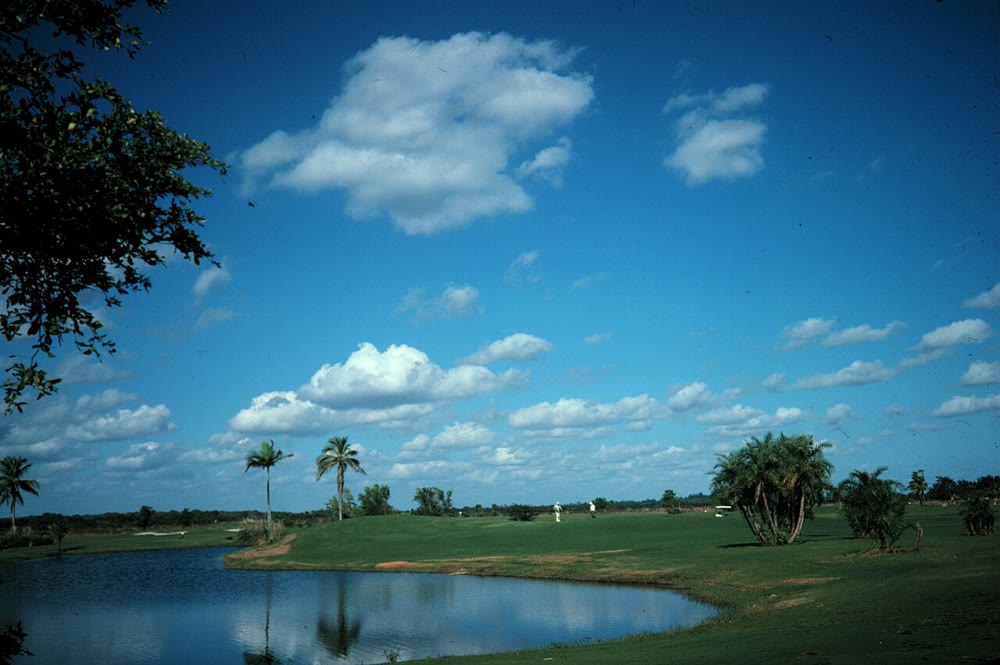
\includegraphics[height=4.5cm]{images/book2/g10-noaa-fair-weather-cumulus.jpg}\hspace{0.6em}%
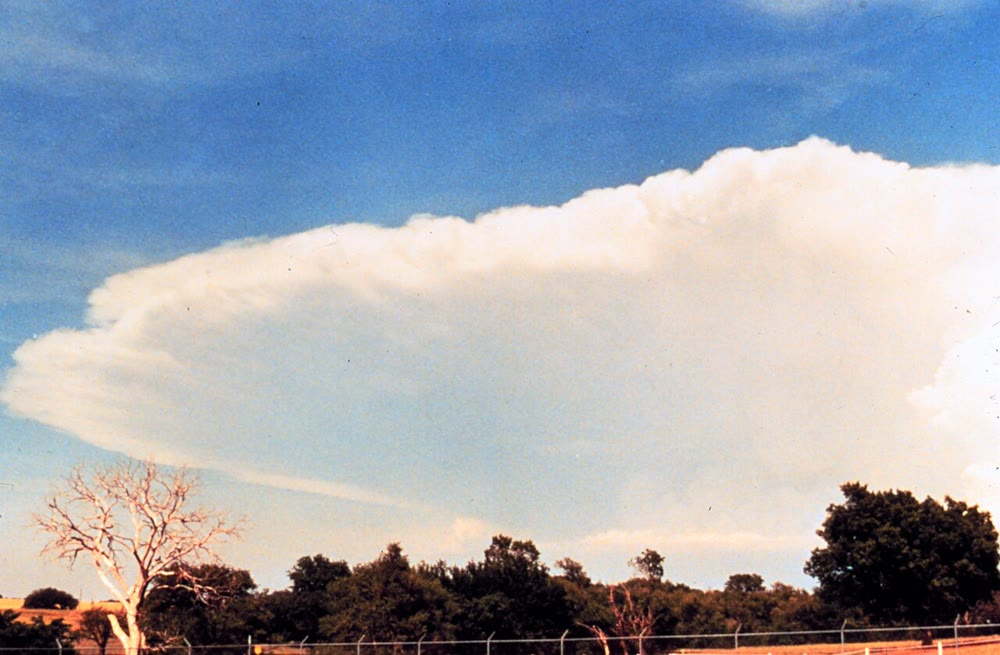
\includegraphics[height=4.5cm]{images/book2/g10-noaa-cumulonimbus-anvil.jpg}

{\small Izquierda: cúmulos de buen tiempo sobre Florida, con su base plana
en el \omterm{def:g10:why-clouds-form:condensation-level}{nivel de condensación}. Fotografía: Ralph F. Kresge, NOAA (dominio
público). Derecha: el yunque de un cumulonimbo en las primeras fases de una
tormenta. Fotografía: NOAA National Severe Storms Laboratory (dominio
público).}
\end{omfigure}

\section{Cuatro maneras de elevar el aire}

El aire sube por cuatro razones.
\begin{itemize}
  \item \textbf{El calentamiento desde abajo.} En un día soleado, el suelo
        calienta el aire que tiene encima; desde las zonas más calientes
        suben burbujas de aire caliente. Son las que dan los cúmulos de la
        tarde.
  \item \textbf{Las montañas.} El viento que sopla contra una cordillera se
        ve obligado a subir por su ladera.
  \item \textbf{Los frentes.} Donde se encuentran masas de aire cálido y
        frío, el aire cálido, más ligero, sube por encima del frío, o el aire
        frío se mete por debajo de él (Libro 1, año 8).
  \item \textbf{La convergencia.} Cuando los vientos confluyen cerca del
        suelo, el aire no tiene más salida que hacia arriba, como en la
        franja de aire ascendente cercana al ecuador y en el centro de una
        borrasca.
\end{itemize}

\begin{method}[Seguir una porción de aire sobre una montaña]\label{met:g10:why-clouds-form:mountain}
\begin{enumerate}
  \item Halla el \omterm{def:g10:why-clouds-form:condensation-level}{nivel de condensación} con la regla de los 125 metros; hasta
        él, la porción se enfría a \qty{9.8}{\degreeCelsius/km}.
  \item Desde allí hasta la cresta se enfría según el gradiente \omterm{def:g10:why-clouds-form:humidity}{saturado}; el
        agua que se condensa cae como lluvia o nieve en la ladera de
        barlovento.
  \item Pasada la cresta, la porción desciende sin estar saturada: se
        calienta a \qty{9.8}{\degreeCelsius/km} durante todo el descenso.
\end{enumerate}
\end{method}

\begin{example}[El viento cálido y seco de sotavento]\label{ex:g10:why-clouds-form:lee}
% ledger: iapws:vapour-pressure, nist:water-latent (all values computed in figdata/grade-10/clouds.py)
Un aire a nivel del mar a \qty{20}{\degreeCelsius}, con un \omterm{def:g10:why-clouds-form:dew-point}{punto de rocío}
de \qty{12}{\degreeCelsius}, es empujado sobre una sierra de \qty{2500}{m}
de altura. Se satura a $125 \times 8 = \qty{1000}{m}$, a unos
\qty{10}{\degreeCelsius}. Desde allí hasta la cresta se enfría según el
gradiente \omterm{def:g10:why-clouds-form:humidity}{saturado}, hasta unos \qty{2}{\degreeCelsius}, y pierde en forma de
lluvia alrededor de un tercio de su agua (de \num{8.7} a \qty{6.0}{g/kg}).
Al bajar por el otro lado se calienta según el gradiente seco a lo largo de
\qty{2.5}{km}: llega a la llanura a unos \qty{27}{\degreeCelsius}, siete
grados más caliente que al principio, con una \omterm{def:g10:why-clouds-form:humidity}{humedad relativa} de alrededor
del \qty{27}{\percent}. Vientos cálidos y secos de este tipo soplan a
sotavento de muchas cordilleras.
\end{example}

\begin{omfigure}
\begin{tikzpicture}[font=\footnotesize, >={Stealth[length=2mm]}]
  \fill[omExo!30] (0,0) -- (3.5,0.3) -- (6,3.0) -- (8.5,0.3) -- (12,0) -- (12,-0.25) -- (0,-0.25) -- cycle;
  \draw[thick, black!70] (0,0) -- (3.5,0.3) -- (6,3.0) -- (8.5,0.3) -- (12,0);
  \draw[black!40, dashed] (0,1.2) -- (4.6,1.2);
  \node[anchor=south west, black!60, align=left] at (0.1,1.22) {nivel de\\condensación, \qty{1000}{m}};
  \foreach \x in {3.62,3.86,4.1} \draw[omDef!60] (\x,1.2) -- (\x-0.06,{0.3+(\x-0.06-3.5)*1.08+0.04});
  \pic[scale=1.1, transform shape] at (4.6,1.22) {puffycloud};
  \pic[scale=0.9, transform shape] at (5.0,2.2) {puffycloud};
  \draw[->, thick, omDef!80!black] (0.2,0.25) -- (2.8,0.5) .. controls (3.6,0.75) .. (4.4,1.7) -- (5.4,2.9) .. controls (5.8,3.4) and (6.2,3.4) .. (6.6,2.9) -- (7.6,1.7) .. controls (8.4,0.75) .. (9.2,0.5) -- (11.8,0.25);
  \node[anchor=east, align=right] at (3.4,2.15) {\qty{10}{\degreeCelsius}, saturado};
  \node[anchor=south, align=center] at (6.0,3.45) {cresta \qty{2500}{m}: \qty{2}{\degreeCelsius}};
  \node[anchor=west, align=left] at (7.75,2.1) {baja y se calienta\\a \qty{9.8}{\degreeCelsius/km}};
  \node[anchor=north, align=center] at (1.0,-0.3) {\qty{20}{\degreeCelsius}\\punto de rocío \qty{12}{\degreeCelsius}};
  \node[anchor=north, align=center] at (11.0,-0.3) {\qty{27}{\degreeCelsius}\\punto de rocío \qty{6}{\degreeCelsius}};
  \node[anchor=north, black!60] at (4.0,-0.3) {barlovento: lluvia};
  \node[anchor=north, black!60] at (8.2,-0.3) {sotavento: seco};
\end{tikzpicture}

{\small Una porción de aire que atraviesa una sierra (temperaturas
calculadas; escala vertical exagerada). Se enfría según el gradiente seco
hasta su \omterm{def:g10:why-clouds-form:condensation-level}{nivel de condensación}, según el gradiente \omterm{def:g10:why-clouds-form:humidity}{saturado}, más lento, por
encima de él, perdiendo agua en forma de lluvia, y se calienta según el
gradiente seco durante todo el descenso por la ladera de sotavento.}
\end{omfigure}

\section{De las gotitas a la lluvia y la nieve}

El vapor de agua no se condensa con facilidad en un aire perfectamente
limpio. Las gotitas se forman sobre motas de materia.

\begin{definition}[Núcleo de condensación]\label{def:g10:why-clouds-form:nucleus}
Un \emph{núcleo de condensación}\index{nucleo de condensacion@núcleo de condensación}
es una diminuta partícula en suspensión en el aire ---un grano de sal
marina, de polvo, de humo o de hollín--- sobre la que el vapor de agua se
condensa para formar una gotita de nube.
\end{definition}

Un núcleo típico mide unos \qty{0.0002}{mm}, una gotita de nube unos
\qty{0.02}{mm}, una gota de llovizna \qty{0.5}{mm} y una gota de lluvia unos
\qty{2}{mm}. Una gota de lluvia es cien veces más ancha que una gotita de
nube, así que su volumen es $100^3$ veces mayor: hace falta un millón de
gotitas de nube para formar una gota de lluvia. Las gotitas de nube son tan
pequeñas que la más leve corriente ascendente las mantiene en el aire; para
que llueva, las gotitas tienen que crecer cien veces.
% ledger: jpl:drop-sizes

\begin{omfigure}
\begin{tikzpicture}
\begin{axis}[width=0.9\linewidth, height=3.4cm, xmode=log, xmin=1e-4, xmax=10,
  ymin=0, ymax=1, axis y line=none, axis x line*=bottom,
  xlabel={diámetro (mm), escala logarítmica}, tick label style={font=\small},
  label style={font=\small}, clip=false]
\addplot[only marks, mark=*, omDef!85!black, mark size=2.5pt] coordinates {(0.0002,0.3) (0.02,0.3) (0.5,0.3) (2,0.3)};
\node[anchor=south, font=\footnotesize, align=center] at (axis cs:0.0002,0.42) {núcleo de\\condensación};
\node[anchor=south, font=\footnotesize, align=center] at (axis cs:0.02,0.42) {gotita\\de nube};
\node[anchor=south, font=\footnotesize, align=center] at (axis cs:0.5,0.42) {llovizna};
\node[anchor=south, font=\footnotesize, align=center] at (axis cs:2,0.42) {gota\\de lluvia};
\end{axis}
\end{tikzpicture}

{\small Tamaños típicos, en una escala en la que cada paso vale diez veces el
anterior: cada objeto es unas cien veces más ancho que el anterior, salvo la
llovizna. Datos: NASA Jet Propulsion Laboratory.}
\end{omfigure}

Dos procesos las hacen crecer.

\begin{definition}[Proceso de lluvia cálida; proceso de cristales de hielo]\label{def:g10:why-clouds-form:rain-processes}
En el \emph{proceso de lluvia cálida}\index{proceso de lluvia calida@proceso de lluvia cálida},
las gotitas más grandes de una nube caen más deprisa que las pequeñas,
chocan con ellas y se fusionan, creciendo mientras caen. En el
\emph{proceso de cristales de hielo}\index{proceso de cristales de hielo},
en la parte de una nube más fría que \qty{0}{\degreeCelsius}, donde se
mezclan cristales de hielo y gotitas subfundidas (líquidas por debajo de
\qty{0}{\degreeCelsius}), los cristales crecen tomando el vapor que se
evapora de las gotitas; caen como copos de nieve, y se funden en gotas de
lluvia si el aire de debajo está templado.
\end{definition}

El \omterm{def:g10:why-clouds-form:rain-processes}{proceso de cristales de hielo} funciona porque el contenido de \omterm{def:g10:why-clouds-form:humidity}{saturación}
es menor sobre el hielo que sobre el agua líquida a la misma temperatura: a
\qty{-10}{\degreeCelsius}, la presión de vapor de \omterm{def:g10:why-clouds-form:humidity}{saturación} es de
\qty{287}{Pa} sobre el agua y de \qty{260}{Pa} sobre el hielo. Un aire
\omterm{def:g10:why-clouds-form:humidity}{saturado} para las gotitas contiene un \qty{10}{\percent} más de vapor del
que admite el hielo: el vapor se condensa sobre los cristales, y las gotitas
se evaporan para reponerlo.
% ledger: iapws:vapour-pressure, iapws:melt-subl (computed in figdata/grade-10/clouds.py)

\begin{remark}[El calor latente alimenta la tormenta]\label{rem:g10:why-clouds-form:latent}
Cada kilogramo de agua que se condensa en una nube cede al aire unos
\qty{2.5}{MJ}, el \omterm{def:g10:earth-energy-budget:latent-heat}{calor latente} que tomó del mar o del suelo al evaporarse
(\cref{ch:g10:earth-energy-budget}). Este calor es lo que hace que el
gradiente \omterm{def:g10:why-clouds-form:humidity}{saturado} sea más lento que el seco y mantiene en ascenso un
cumulonimbo; el \cref{ch:g10:storms-and-cyclones} lo sigue hasta las
tormentas más grandes.
\end{remark}
% ledger: nist:water-latent

\section{Ejercicios}

Para estos ejercicios, usa los contenidos de \omterm{def:g10:why-clouds-form:humidity}{saturación} (en \unit{g/kg}, a
la presión del nivel del mar) de la tabla siguiente, el gradiente seco de
\qty{9.8}{\degreeCelsius/km}, un descenso del \omterm{def:g10:why-clouds-form:dew-point}{punto de rocío} de
\qty{1.8}{\degreeCelsius/km} y un gradiente \omterm{def:g10:why-clouds-form:humidity}{saturado} de
\qty{5}{\degreeCelsius/km}.
% ledger: iapws:vapour-pressure (table from figdata/out/grade-10-clouds-sat.dat, rounded)

\begin{center}
\small
\begin{tabular}{l*{11}{c}}
\hline
temperatura (\unit{\degreeCelsius}) & 0 & 4 & 8 & 10 & 12 & 14 & 16 & 20 & 24 & 28 & 30 \\
contenido de \omterm{def:g10:why-clouds-form:humidity}{saturación} (\unit{g/kg}) & 3.8 & 5.0 & 6.7 & 7.6 & 8.7 & 10.0 & 11.4 & 14.7 & 18.9 & 24.1 & 27.2 \\
\hline
\end{tabular}
\end{center}

\begin{exercise}[$\star$]\label{exo:g10:why-clouds-form:1}
Define la \omterm{def:g10:why-clouds-form:humidity}{humedad relativa} y el \omterm{def:g10:why-clouds-form:dew-point}{punto de rocío} del aire.
\end{exercise}

\begin{exercise}[$\star$]\label{exo:g10:why-clouds-form:2}
A partir de la tabla, da el contenido de \omterm{def:g10:why-clouds-form:humidity}{saturación} a \num{0}, \num{10},
\num{20} y \qty{30}{\degreeCelsius}. ¿Aproximadamente por qué factor aumenta
por cada \qty{10}{\degreeCelsius} de calentamiento?
\end{exercise}

\begin{exercise}[$\star$]\label{exo:g10:why-clouds-form:3}
Un aire a \qty{24}{\degreeCelsius} contiene \qty{10.0}{g/kg} de vapor de
agua. Halla su \omterm{def:g10:why-clouds-form:humidity}{humedad relativa} y su \omterm{def:g10:why-clouds-form:dew-point}{punto de rocío}.
\end{exercise}

\begin{exercise}[$\star$]\label{exo:g10:why-clouds-form:4}
Explica por qué un vaso de agua con hielo ``suda'' en verano, y por qué no
lo hace en interior un día de invierno muy seco.
\end{exercise}

\begin{exercise}[$\star$]\label{exo:g10:why-clouds-form:5}
Nombra las cuatro maneras de hacer subir el aire, con un ejemplo de cada una.
\end{exercise}

\begin{exercise}[$\star\star$]\label{exo:g10:why-clouds-form:6}
Con la \cref{prop:g10:why-clouds-form:lcl}, halla la altura de la base de
las nubes para un aire a \qty{30}{\degreeCelsius} con un \omterm{def:g10:why-clouds-form:dew-point}{punto de rocío} de
\qty{18}{\degreeCelsius}, y para un aire a \qty{22}{\degreeCelsius} con un
\omterm{def:g10:why-clouds-form:dew-point}{punto de rocío} de \qty{20}{\degreeCelsius}. ¿Qué día es probable que esté
gris y con nubes bajas?
\end{exercise}

\begin{exercise}[$\star\star$]\label{exo:g10:why-clouds-form:7}
Una porción de aire no \omterm{def:g10:why-clouds-form:humidity}{saturado} sale del suelo a \qty{18}{\degreeCelsius}.
¿Cuál es su temperatura a \qty{1}{km} y a \qty{2}{km} de altura, si sigue
sin saturarse? Si vuelve a bajar desde \qty{2}{km}, ¿a qué temperatura llega
al suelo?
\end{exercise}

\begin{exercise}[$\star\star$]\label{exo:g10:why-clouds-form:8}
Un sondeo en globo muestra que la temperatura baja \qty{4}{\degreeCelsius}
por km. ¿Es \omterm{def:g10:why-clouds-form:stability}{estable} el aire para una porción no saturada? ¿Y para una
saturada? Una tarde calurosa, la temperatura baja \qty{12}{\degreeCelsius} en
el primer kilómetro por encima del suelo: ¿qué les ocurre a las burbujas de
aire caliente?
\end{exercise}

\begin{exercise}[$\star\star$]\label{exo:g10:why-clouds-form:9}
Un aire \omterm{def:g10:why-clouds-form:humidity}{saturado} a \qty{20}{\degreeCelsius} se enfría hasta
\qty{10}{\degreeCelsius}. ¿Cuántos gramos de agua se condensan por kilogramo
de aire? ¿Adónde va el \omterm{def:g10:earth-energy-budget:latent-heat}{calor latente} liberado?
\end{exercise}

\begin{exercise}[$\star\star$]\label{exo:g10:why-clouds-form:10}
¿Cuántas gotitas de nube de \qty{0.02}{mm} de diámetro forman una gota de
llovizna de \qty{0.5}{mm} de diámetro? ¿Y una gota de lluvia de
\qty{2}{mm}?
\end{exercise}

\begin{exercise}[$\star\star$]\label{exo:g10:why-clouds-form:11}
Explica, paso a paso, por qué al amanecer, después de una noche despejada y
en calma, la niebla se forma en los valles y no en las cimas de las colinas.
\end{exercise}

\begin{exercise}[$\star\star\star$]\label{exo:g10:why-clouds-form:12}
El gradiente seco es $a$ y el \omterm{def:g10:why-clouds-form:dew-point}{punto de rocío} baja a un ritmo $b$ (ambos en
\unit{\degreeCelsius/km}). Demuestra que el \omterm{def:g10:why-clouds-form:condensation-level}{nivel de condensación} está a
$z = (T - T_d)/(a - b)$. Sobre una meseta alta, el \omterm{def:g10:why-clouds-form:dew-point}{punto de rocío} baja
\qty{1.7}{\degreeCelsius/km}: ¿en qué se convierte la regla de los
``\qty{125}{m} por grado''?
\end{exercise}

\begin{exercise}[$\star\star\star$]\label{exo:g10:why-clouds-form:13}
Un aire a nivel del mar a \qty{15}{\degreeCelsius}, con un \omterm{def:g10:why-clouds-form:dew-point}{punto de rocío} de
\qty{11}{\degreeCelsius}, atraviesa una sierra de \qty{2000}{m} de altura.
Siguiendo el \cref{met:g10:why-clouds-form:mountain}, halla el \omterm{def:g10:why-clouds-form:condensation-level}{nivel de
condensación}, la temperatura a ese nivel, la temperatura en la cresta y la
temperatura con la que el aire llega a la llanura del otro lado.
\end{exercise}

\begin{exercise}[$\star\star\star$]\label{exo:g10:why-clouds-form:14}
A \qty{-20}{\degreeCelsius}, la presión de vapor de \omterm{def:g10:why-clouds-form:humidity}{saturación} es de
\qty{126}{Pa} sobre el agua y de \qty{103}{Pa} sobre el hielo. ¿En qué
porcentaje está sobresaturado respecto al hielo un aire \omterm{def:g10:why-clouds-form:humidity}{saturado} para las
gotitas? Compáralo con \qty{-10}{\degreeCelsius}, y di en qué parte de una
nube funciona mejor el \omterm{def:g10:why-clouds-form:rain-processes}{proceso de cristales de hielo}.
\end{exercise}

\begin{exercise}[$\star\star\star$]\label{exo:g10:why-clouds-form:15}
El aire del entorno se enfría \qty{6.5}{\degreeCelsius/km}. Una porción sale
a la misma temperatura que su entorno y sube \qty{1}{km}. Calcula la
diferencia entre su temperatura y la del entorno si no está saturada, y
después si está saturada. Explica la expresión ``condicionalmente
\omterm{def:g10:why-clouds-form:stability}{inestable}''.
\end{exercise}

\section{Problema: una tarde de verano sobre la llanura}

\begin{problem}[{Problema de fin de semana --- de la humedad de la mañana a
la base de las nubes de la tarde}]
\label{pb:g10:why-clouds-form:1}
% ledger: iapws:vapour-pressure, nist:water-latent (all results computed in figdata/grade-10/clouds.py or from the rounded data below; the sounding is sounding A, invented)
Sobre una amplia llanura, un día de verano, el aire cercano al suelo
contiene \qty{11.4}{g/kg} de vapor de agua durante todo el día. Está a
\qty{20}{\degreeCelsius} por la mañana y a \qty{28}{\degreeCelsius} por la
tarde. Un sondeo en globo (un ejemplo inventado) da la temperatura del aire
de las capas superiores:

\begin{center}
\small
\begin{tabular}{l*{8}{c}}
\hline
altura (km) & 0 & 0.5 & 1.0 & 1.5 & 2.5 & 3.5 & 3.6 & 4.0 \\
temperatura (\unit{\degreeCelsius}) & 28.0 & 23.1 & 18.2 & 13.4 & 6.9 & 0.4 & $-0.3$ & 1.2 \\
\hline
\end{tabular}
\end{center}

\noindent Usa la tabla de contenidos de \omterm{def:g10:why-clouds-form:humidity}{saturación} y los ritmos dados antes
de los ejercicios.

\medskip
\noindent\textbf{Parte I --- La humedad.}
\begin{enumerate}
  \item Da el contenido de \omterm{def:g10:why-clouds-form:humidity}{saturación} a \qty{20}{\degreeCelsius}.
  \item Calcula la \omterm{def:g10:why-clouds-form:humidity}{humedad relativa} de la mañana.
  \item Halla el \omterm{def:g10:why-clouds-form:dew-point}{punto de rocío} del aire.
  \item Calcula la \omterm{def:g10:why-clouds-form:humidity}{humedad relativa} por la tarde.
  \item ¿Se ha vuelto más seco el aire por la tarde? Explícalo.
\end{enumerate}

\medskip
\noindent\textbf{Parte II --- La noche y el rocío.}
\begin{enumerate}[resume]
  \item Durante la noche, el aire cercano al suelo se enfría. ¿A qué
        temperatura empieza a formarse rocío?
  \item Si el aire se enfría hasta \qty{12}{\degreeCelsius}, ¿cuántos gramos
        de agua por kilogramo de aire se han condensado?
  \item ¿Por qué se forma el rocío sobre la hierba y sobre los techos de los
        coches antes que en el aire?
\end{enumerate}

\medskip
\noindent\textbf{Parte III --- El sondeo.}
\begin{enumerate}[resume]
  \item Calcula el ritmo al que baja la temperatura entre \num{0} y
        \qty{1.5}{km}. Compáralo con el gradiente seco.
  \item Calcúlalo entre \num{1.5} y \qty{3.5}{km}.
  \item ¿Es \omterm{def:g10:why-clouds-form:stability}{estable} el aire entre \num{1.5} y \qty{3.5}{km} para una porción
        no saturada? ¿Y para una saturada?
  \item ¿Qué ocurre entre \num{3.6} y \qty{4.0}{km}? ¿Qué efecto tiene sobre
        una nube que crece hacia arriba?
\end{enumerate}

\medskip
\noindent\textbf{Parte IV --- La base de las nubes.}
\begin{enumerate}[resume]
  \item Calcula la diferencia entre la temperatura del aire y su \omterm{def:g10:why-clouds-form:dew-point}{punto de
        rocío} junto al suelo por la tarde.
  \item Calcula la temperatura y el \omterm{def:g10:why-clouds-form:dew-point}{punto de rocío} de una burbuja de este
        aire después de subir \qty{1}{km}, todavía sin saturar.
  \item ¿Cuánto se ha reducido la diferencia entre ambos? ¿A qué ritmo se
        reduce?
  \item Demuestra que este ritmo da la regla de los ``\qty{125}{m} por
        grado''.
  \item ¿A qué altura habría estado la base de las nubes por la mañana?
  \item Explica por qué la base de los cúmulos sube a lo largo del día.
  \item Escribe la ecuación que expresa que la temperatura de la burbuja es
        igual a su \omterm{def:g10:why-clouds-form:dew-point}{punto de rocío} a la altura $z$ (en km).
  \item Resuélvela: ¿a qué altura está la base de los cúmulos de la tarde?
\end{enumerate}
\end{problem}
